
\documentclass{article} % For LaTeX2e
\usepackage{iclr2021_conference,times}

% Optional math commands from https://github.com/goodfeli/dlbook_notation.
%%%%% NEW MATH DEFINITIONS %%%%%

\usepackage{amsmath,amsfonts,bm}

% Mark sections of captions for referring to divisions of figures
\newcommand{\figleft}{{\em (Left)}}
\newcommand{\figcenter}{{\em (Center)}}
\newcommand{\figright}{{\em (Right)}}
\newcommand{\figtop}{{\em (Top)}}
\newcommand{\figbottom}{{\em (Bottom)}}
\newcommand{\captiona}{{\em (a)}}
\newcommand{\captionb}{{\em (b)}}
\newcommand{\captionc}{{\em (c)}}
\newcommand{\captiond}{{\em (d)}}

% Highlight a newly defined term
\newcommand{\newterm}[1]{{\bf #1}}


% Figure reference, lower-case.
\def\figref#1{figure~\ref{#1}}
% Figure reference, capital. For start of sentence
\def\Figref#1{Figure~\ref{#1}}
\def\twofigref#1#2{figures \ref{#1} and \ref{#2}}
\def\quadfigref#1#2#3#4{figures \ref{#1}, \ref{#2}, \ref{#3} and \ref{#4}}
% Section reference, lower-case.
\def\secref#1{section~\ref{#1}}
% Section reference, capital.
\def\Secref#1{Section~\ref{#1}}
% Reference to two sections.
\def\twosecrefs#1#2{sections \ref{#1} and \ref{#2}}
% Reference to three sections.
\def\secrefs#1#2#3{sections \ref{#1}, \ref{#2} and \ref{#3}}
% Reference to an equation, lower-case.
\def\eqref#1{equation~\ref{#1}}
% Reference to an equation, upper case
\def\Eqref#1{Equation~\ref{#1}}
% A raw reference to an equation---avoid using if possible
\def\plaineqref#1{\ref{#1}}
% Reference to a chapter, lower-case.
\def\chapref#1{chapter~\ref{#1}}
% Reference to an equation, upper case.
\def\Chapref#1{Chapter~\ref{#1}}
% Reference to a range of chapters
\def\rangechapref#1#2{chapters\ref{#1}--\ref{#2}}
% Reference to an algorithm, lower-case.
\def\algref#1{algorithm~\ref{#1}}
% Reference to an algorithm, upper case.
\def\Algref#1{Algorithm~\ref{#1}}
\def\twoalgref#1#2{algorithms \ref{#1} and \ref{#2}}
\def\Twoalgref#1#2{Algorithms \ref{#1} and \ref{#2}}
% Reference to a part, lower case
\def\partref#1{part~\ref{#1}}
% Reference to a part, upper case
\def\Partref#1{Part~\ref{#1}}
\def\twopartref#1#2{parts \ref{#1} and \ref{#2}}

\def\ceil#1{\lceil #1 \rceil}
\def\floor#1{\lfloor #1 \rfloor}
\def\1{\bm{1}}
\newcommand{\train}{\mathcal{D}}
\newcommand{\valid}{\mathcal{D_{\mathrm{valid}}}}
\newcommand{\test}{\mathcal{D_{\mathrm{test}}}}

\def\eps{{\epsilon}}


% Random variables
\def\reta{{\textnormal{$\eta$}}}
\def\ra{{\textnormal{a}}}
\def\rb{{\textnormal{b}}}
\def\rc{{\textnormal{c}}}
\def\rd{{\textnormal{d}}}
\def\re{{\textnormal{e}}}
\def\rf{{\textnormal{f}}}
\def\rg{{\textnormal{g}}}
\def\rh{{\textnormal{h}}}
\def\ri{{\textnormal{i}}}
\def\rj{{\textnormal{j}}}
\def\rk{{\textnormal{k}}}
\def\rl{{\textnormal{l}}}
% rm is already a command, just don't name any random variables m
\def\rn{{\textnormal{n}}}
\def\ro{{\textnormal{o}}}
\def\rp{{\textnormal{p}}}
\def\rq{{\textnormal{q}}}
\def\rr{{\textnormal{r}}}
\def\rs{{\textnormal{s}}}
\def\rt{{\textnormal{t}}}
\def\ru{{\textnormal{u}}}
\def\rv{{\textnormal{v}}}
\def\rw{{\textnormal{w}}}
\def\rx{{\textnormal{x}}}
\def\ry{{\textnormal{y}}}
\def\rz{{\textnormal{z}}}

% Random vectors
\def\rvepsilon{{\mathbf{\epsilon}}}
\def\rvtheta{{\mathbf{\theta}}}
\def\rva{{\mathbf{a}}}
\def\rvb{{\mathbf{b}}}
\def\rvc{{\mathbf{c}}}
\def\rvd{{\mathbf{d}}}
\def\rve{{\mathbf{e}}}
\def\rvf{{\mathbf{f}}}
\def\rvg{{\mathbf{g}}}
\def\rvh{{\mathbf{h}}}
\def\rvu{{\mathbf{i}}}
\def\rvj{{\mathbf{j}}}
\def\rvk{{\mathbf{k}}}
\def\rvl{{\mathbf{l}}}
\def\rvm{{\mathbf{m}}}
\def\rvn{{\mathbf{n}}}
\def\rvo{{\mathbf{o}}}
\def\rvp{{\mathbf{p}}}
\def\rvq{{\mathbf{q}}}
\def\rvr{{\mathbf{r}}}
\def\rvs{{\mathbf{s}}}
\def\rvt{{\mathbf{t}}}
\def\rvu{{\mathbf{u}}}
\def\rvv{{\mathbf{v}}}
\def\rvw{{\mathbf{w}}}
\def\rvx{{\mathbf{x}}}
\def\rvy{{\mathbf{y}}}
\def\rvz{{\mathbf{z}}}

% Elements of random vectors
\def\erva{{\textnormal{a}}}
\def\ervb{{\textnormal{b}}}
\def\ervc{{\textnormal{c}}}
\def\ervd{{\textnormal{d}}}
\def\erve{{\textnormal{e}}}
\def\ervf{{\textnormal{f}}}
\def\ervg{{\textnormal{g}}}
\def\ervh{{\textnormal{h}}}
\def\ervi{{\textnormal{i}}}
\def\ervj{{\textnormal{j}}}
\def\ervk{{\textnormal{k}}}
\def\ervl{{\textnormal{l}}}
\def\ervm{{\textnormal{m}}}
\def\ervn{{\textnormal{n}}}
\def\ervo{{\textnormal{o}}}
\def\ervp{{\textnormal{p}}}
\def\ervq{{\textnormal{q}}}
\def\ervr{{\textnormal{r}}}
\def\ervs{{\textnormal{s}}}
\def\ervt{{\textnormal{t}}}
\def\ervu{{\textnormal{u}}}
\def\ervv{{\textnormal{v}}}
\def\ervw{{\textnormal{w}}}
\def\ervx{{\textnormal{x}}}
\def\ervy{{\textnormal{y}}}
\def\ervz{{\textnormal{z}}}

% Random matrices
\def\rmA{{\mathbf{A}}}
\def\rmB{{\mathbf{B}}}
\def\rmC{{\mathbf{C}}}
\def\rmD{{\mathbf{D}}}
\def\rmE{{\mathbf{E}}}
\def\rmF{{\mathbf{F}}}
\def\rmG{{\mathbf{G}}}
\def\rmH{{\mathbf{H}}}
\def\rmI{{\mathbf{I}}}
\def\rmJ{{\mathbf{J}}}
\def\rmK{{\mathbf{K}}}
\def\rmL{{\mathbf{L}}}
\def\rmM{{\mathbf{M}}}
\def\rmN{{\mathbf{N}}}
\def\rmO{{\mathbf{O}}}
\def\rmP{{\mathbf{P}}}
\def\rmQ{{\mathbf{Q}}}
\def\rmR{{\mathbf{R}}}
\def\rmS{{\mathbf{S}}}
\def\rmT{{\mathbf{T}}}
\def\rmU{{\mathbf{U}}}
\def\rmV{{\mathbf{V}}}
\def\rmW{{\mathbf{W}}}
\def\rmX{{\mathbf{X}}}
\def\rmY{{\mathbf{Y}}}
\def\rmZ{{\mathbf{Z}}}

% Elements of random matrices
\def\ermA{{\textnormal{A}}}
\def\ermB{{\textnormal{B}}}
\def\ermC{{\textnormal{C}}}
\def\ermD{{\textnormal{D}}}
\def\ermE{{\textnormal{E}}}
\def\ermF{{\textnormal{F}}}
\def\ermG{{\textnormal{G}}}
\def\ermH{{\textnormal{H}}}
\def\ermI{{\textnormal{I}}}
\def\ermJ{{\textnormal{J}}}
\def\ermK{{\textnormal{K}}}
\def\ermL{{\textnormal{L}}}
\def\ermM{{\textnormal{M}}}
\def\ermN{{\textnormal{N}}}
\def\ermO{{\textnormal{O}}}
\def\ermP{{\textnormal{P}}}
\def\ermQ{{\textnormal{Q}}}
\def\ermR{{\textnormal{R}}}
\def\ermS{{\textnormal{S}}}
\def\ermT{{\textnormal{T}}}
\def\ermU{{\textnormal{U}}}
\def\ermV{{\textnormal{V}}}
\def\ermW{{\textnormal{W}}}
\def\ermX{{\textnormal{X}}}
\def\ermY{{\textnormal{Y}}}
\def\ermZ{{\textnormal{Z}}}

% Vectors
\def\vzero{{\bm{0}}}
\def\vone{{\bm{1}}}
\def\vmu{{\bm{\mu}}}
\def\vtheta{{\bm{\theta}}}
\def\va{{\bm{a}}}
\def\vb{{\bm{b}}}
\def\vc{{\bm{c}}}
\def\vd{{\bm{d}}}
\def\ve{{\bm{e}}}
\def\vf{{\bm{f}}}
\def\vg{{\bm{g}}}
\def\vh{{\bm{h}}}
\def\vi{{\bm{i}}}
\def\vj{{\bm{j}}}
\def\vk{{\bm{k}}}
\def\vl{{\bm{l}}}
\def\vm{{\bm{m}}}
\def\vn{{\bm{n}}}
\def\vo{{\bm{o}}}
\def\vp{{\bm{p}}}
\def\vq{{\bm{q}}}
\def\vr{{\bm{r}}}
\def\vs{{\bm{s}}}
\def\vt{{\bm{t}}}
\def\vu{{\bm{u}}}
\def\vv{{\bm{v}}}
\def\vw{{\bm{w}}}
\def\vx{{\bm{x}}}
\def\vy{{\bm{y}}}
\def\vz{{\bm{z}}}

% Elements of vectors
\def\evalpha{{\alpha}}
\def\evbeta{{\beta}}
\def\evepsilon{{\epsilon}}
\def\evlambda{{\lambda}}
\def\evomega{{\omega}}
\def\evmu{{\mu}}
\def\evpsi{{\psi}}
\def\evsigma{{\sigma}}
\def\evtheta{{\theta}}
\def\eva{{a}}
\def\evb{{b}}
\def\evc{{c}}
\def\evd{{d}}
\def\eve{{e}}
\def\evf{{f}}
\def\evg{{g}}
\def\evh{{h}}
\def\evi{{i}}
\def\evj{{j}}
\def\evk{{k}}
\def\evl{{l}}
\def\evm{{m}}
\def\evn{{n}}
\def\evo{{o}}
\def\evp{{p}}
\def\evq{{q}}
\def\evr{{r}}
\def\evs{{s}}
\def\evt{{t}}
\def\evu{{u}}
\def\evv{{v}}
\def\evw{{w}}
\def\evx{{x}}
\def\evy{{y}}
\def\evz{{z}}

% Matrix
\def\mA{{\bm{A}}}
\def\mB{{\bm{B}}}
\def\mC{{\bm{C}}}
\def\mD{{\bm{D}}}
\def\mE{{\bm{E}}}
\def\mF{{\bm{F}}}
\def\mG{{\bm{G}}}
\def\mH{{\bm{H}}}
\def\mI{{\bm{I}}}
\def\mJ{{\bm{J}}}
\def\mK{{\bm{K}}}
\def\mL{{\bm{L}}}
\def\mM{{\bm{M}}}
\def\mN{{\bm{N}}}
\def\mO{{\bm{O}}}
\def\mP{{\bm{P}}}
\def\mQ{{\bm{Q}}}
\def\mR{{\bm{R}}}
\def\mS{{\bm{S}}}
\def\mT{{\bm{T}}}
\def\mU{{\bm{U}}}
\def\mV{{\bm{V}}}
\def\mW{{\bm{W}}}
\def\mX{{\bm{X}}}
\def\mY{{\bm{Y}}}
\def\mZ{{\bm{Z}}}
\def\mBeta{{\bm{\beta}}}
\def\mPhi{{\bm{\Phi}}}
\def\mLambda{{\bm{\Lambda}}}
\def\mSigma{{\bm{\Sigma}}}

% Tensor
\DeclareMathAlphabet{\mathsfit}{\encodingdefault}{\sfdefault}{m}{sl}
\SetMathAlphabet{\mathsfit}{bold}{\encodingdefault}{\sfdefault}{bx}{n}
\newcommand{\tens}[1]{\bm{\mathsfit{#1}}}
\def\tA{{\tens{A}}}
\def\tB{{\tens{B}}}
\def\tC{{\tens{C}}}
\def\tD{{\tens{D}}}
\def\tE{{\tens{E}}}
\def\tF{{\tens{F}}}
\def\tG{{\tens{G}}}
\def\tH{{\tens{H}}}
\def\tI{{\tens{I}}}
\def\tJ{{\tens{J}}}
\def\tK{{\tens{K}}}
\def\tL{{\tens{L}}}
\def\tM{{\tens{M}}}
\def\tN{{\tens{N}}}
\def\tO{{\tens{O}}}
\def\tP{{\tens{P}}}
\def\tQ{{\tens{Q}}}
\def\tR{{\tens{R}}}
\def\tS{{\tens{S}}}
\def\tT{{\tens{T}}}
\def\tU{{\tens{U}}}
\def\tV{{\tens{V}}}
\def\tW{{\tens{W}}}
\def\tX{{\tens{X}}}
\def\tY{{\tens{Y}}}
\def\tZ{{\tens{Z}}}


% Graph
\def\gA{{\mathcal{A}}}
\def\gB{{\mathcal{B}}}
\def\gC{{\mathcal{C}}}
\def\gD{{\mathcal{D}}}
\def\gE{{\mathcal{E}}}
\def\gF{{\mathcal{F}}}
\def\gG{{\mathcal{G}}}
\def\gH{{\mathcal{H}}}
\def\gI{{\mathcal{I}}}
\def\gJ{{\mathcal{J}}}
\def\gK{{\mathcal{K}}}
\def\gL{{\mathcal{L}}}
\def\gM{{\mathcal{M}}}
\def\gN{{\mathcal{N}}}
\def\gO{{\mathcal{O}}}
\def\gP{{\mathcal{P}}}
\def\gQ{{\mathcal{Q}}}
\def\gR{{\mathcal{R}}}
\def\gS{{\mathcal{S}}}
\def\gT{{\mathcal{T}}}
\def\gU{{\mathcal{U}}}
\def\gV{{\mathcal{V}}}
\def\gW{{\mathcal{W}}}
\def\gX{{\mathcal{X}}}
\def\gY{{\mathcal{Y}}}
\def\gZ{{\mathcal{Z}}}

% Sets
\def\sA{{\mathbb{A}}}
\def\sB{{\mathbb{B}}}
\def\sC{{\mathbb{C}}}
\def\sD{{\mathbb{D}}}
% Don't use a set called E, because this would be the same as our symbol
% for expectation.
\def\sF{{\mathbb{F}}}
\def\sG{{\mathbb{G}}}
\def\sH{{\mathbb{H}}}
\def\sI{{\mathbb{I}}}
\def\sJ{{\mathbb{J}}}
\def\sK{{\mathbb{K}}}
\def\sL{{\mathbb{L}}}
\def\sM{{\mathbb{M}}}
\def\sN{{\mathbb{N}}}
\def\sO{{\mathbb{O}}}
\def\sP{{\mathbb{P}}}
\def\sQ{{\mathbb{Q}}}
\def\sR{{\mathbb{R}}}
\def\sS{{\mathbb{S}}}
\def\sT{{\mathbb{T}}}
\def\sU{{\mathbb{U}}}
\def\sV{{\mathbb{V}}}
\def\sW{{\mathbb{W}}}
\def\sX{{\mathbb{X}}}
\def\sY{{\mathbb{Y}}}
\def\sZ{{\mathbb{Z}}}

% Entries of a matrix
\def\emLambda{{\Lambda}}
\def\emA{{A}}
\def\emB{{B}}
\def\emC{{C}}
\def\emD{{D}}
\def\emE{{E}}
\def\emF{{F}}
\def\emG{{G}}
\def\emH{{H}}
\def\emI{{I}}
\def\emJ{{J}}
\def\emK{{K}}
\def\emL{{L}}
\def\emM{{M}}
\def\emN{{N}}
\def\emO{{O}}
\def\emP{{P}}
\def\emQ{{Q}}
\def\emR{{R}}
\def\emS{{S}}
\def\emT{{T}}
\def\emU{{U}}
\def\emV{{V}}
\def\emW{{W}}
\def\emX{{X}}
\def\emY{{Y}}
\def\emZ{{Z}}
\def\emSigma{{\Sigma}}

% entries of a tensor
% Same font as tensor, without \bm wrapper
\newcommand{\etens}[1]{\mathsfit{#1}}
\def\etLambda{{\etens{\Lambda}}}
\def\etA{{\etens{A}}}
\def\etB{{\etens{B}}}
\def\etC{{\etens{C}}}
\def\etD{{\etens{D}}}
\def\etE{{\etens{E}}}
\def\etF{{\etens{F}}}
\def\etG{{\etens{G}}}
\def\etH{{\etens{H}}}
\def\etI{{\etens{I}}}
\def\etJ{{\etens{J}}}
\def\etK{{\etens{K}}}
\def\etL{{\etens{L}}}
\def\etM{{\etens{M}}}
\def\etN{{\etens{N}}}
\def\etO{{\etens{O}}}
\def\etP{{\etens{P}}}
\def\etQ{{\etens{Q}}}
\def\etR{{\etens{R}}}
\def\etS{{\etens{S}}}
\def\etT{{\etens{T}}}
\def\etU{{\etens{U}}}
\def\etV{{\etens{V}}}
\def\etW{{\etens{W}}}
\def\etX{{\etens{X}}}
\def\etY{{\etens{Y}}}
\def\etZ{{\etens{Z}}}

% The true underlying data generating distribution
\newcommand{\pdata}{p_{\rm{data}}}
% The empirical distribution defined by the training set
\newcommand{\ptrain}{\hat{p}_{\rm{data}}}
\newcommand{\Ptrain}{\hat{P}_{\rm{data}}}
% The model distribution
\newcommand{\pmodel}{p_{\rm{model}}}
\newcommand{\Pmodel}{P_{\rm{model}}}
\newcommand{\ptildemodel}{\tilde{p}_{\rm{model}}}
% Stochastic autoencoder distributions
\newcommand{\pencode}{p_{\rm{encoder}}}
\newcommand{\pdecode}{p_{\rm{decoder}}}
\newcommand{\precons}{p_{\rm{reconstruct}}}

\newcommand{\laplace}{\mathrm{Laplace}} % Laplace distribution

\newcommand{\E}{\mathbb{E}}
\newcommand{\Ls}{\mathcal{L}}
\newcommand{\R}{\mathbb{R}}
\newcommand{\emp}{\tilde{p}}
\newcommand{\lr}{\alpha}
\newcommand{\reg}{\lambda}
\newcommand{\rect}{\mathrm{rectifier}}
\newcommand{\softmax}{\mathrm{softmax}}
\newcommand{\sigmoid}{\sigma}
\newcommand{\softplus}{\zeta}
\newcommand{\KL}{D_{\mathrm{KL}}}
\newcommand{\Var}{\mathrm{Var}}
\newcommand{\standarderror}{\mathrm{SE}}
\newcommand{\Cov}{\mathrm{Cov}}
% Wolfram Mathworld says $L^2$ is for function spaces and $\ell^2$ is for vectors
% But then they seem to use $L^2$ for vectors throughout the site, and so does
% wikipedia.
\newcommand{\normlzero}{L^0}
\newcommand{\normlone}{L^1}
\newcommand{\normltwo}{L^2}
\newcommand{\normlp}{L^p}
\newcommand{\normmax}{L^\infty}

\newcommand{\parents}{Pa} % See usage in notation.tex. Chosen to match Daphne's book.

\DeclareMathOperator*{\argmax}{arg\,max}
\DeclareMathOperator*{\argmin}{arg\,min}

\DeclareMathOperator{\sign}{sign}
\DeclareMathOperator{\Tr}{Tr}
\let\ab\allowbreak


\usepackage{hyperref}
\usepackage{url}
\usepackage{graphicx}


\title{Neuro 240 Final Project Report - \\Playing Pac-Man Using RL}

% Authors must not appear in the submitted version. They should be hidden
% as long as the \iclrfinalcopy macro remains commented out below.
% Non-anonymous submissions will be rejected without review.

\author{Nicholas Yang\\
\texttt{nyang@college.harvard.edu}}

% The \author macro works with any number of authors. There are two commands
% used to separate the names and addresses of multiple authors: \And and \AND.
%
% Using \And between authors leaves it to \LaTeX{} to determine where to break
% the lines. Using \AND forces a linebreak at that point. So, if \LaTeX{}
% puts 3 of 4 authors names on the first line, and the last on the second
% line, try using \AND instead of \And before the third author name.

\newcommand{\fix}{\marginpar{FIX}}
\newcommand{\new}{\marginpar{NEW}}

\iclrfinalcopy % Uncomment for camera-ready version, but NOT for submission.
\begin{document}


\maketitle

\begin{abstract}
  This project investigates the effectiveness of a Deep Reinforcement Learning (RL) agent, specifically using a Deep Q-Learning algorithm, in navigating a simulated Pac-Man environment characterized by dynamically changing ghost behaviors. We explore how implementing additional improvements to the baseline Deep RL algorithm to improve the model's behavior. We also explore how the variability of ghost strategies impacts the agent's decision-making and overall performance. The agent receives real-time state inputs, including ghost positions, pellet locations, and Pac-Man's coordinates, and outputs optimal directional movements. Our hypothesis posits that the agent can successfully predict and adapt to ghost behaviors resembling previously encountered patterns but struggles with novel strategies, and that the improvements we make to the algorithm will make that model better at adapting to new environments than the original model will. Performance evaluation is based on the highest and average levels reached across multiple trials, offering quantitative insight into the agent's adaptability and robustness. This study provides valuable insights into the capacity and limitations of Deep Q-Learning models in dynamically unpredictable gaming environments.
\end{abstract}

\section{Introduction}

Reinforcement learning has become a way to model how the brain behaves when meeting new information: given some sort of reward function, the model should be able to iteratively learn how to solve a problem by itself. These types of algorithms have proven to learn the best path forward given a finite state space as well as a limited set of potential actions that the agent can take. Atari games, known for their arcade-style themes and simple gameplay dynamics, are a common starting place for testing certain reinforcement learning algorithms to determine efficacy. In particular, games such as Flappy Bird have a finite number of gameplay states (position of the bird and the position of the pillars) as well as a finite number of actions (do nothing and flap). We take another look at a different game: Pac-Man.

The game of Pac-Man involves controlling a character within the game called Pac-Man where the goal of the game is to eat all of the dots in an enclosed maze while avoiding the four ghosts in the maze, each of which have certain behaviors. The Pac-Man character is limited to moving in four directions or not moving at all, proving a finite number of potential moves, and there are a finite number of game states as well since the Pac-Man and the ghosts can only exist in certain locations on the maze.

Scoring primarily occurs through consuming various items scattered across the maze. Pac-Man earns 10 points for each regular pellet (small dot) eaten and 50 points for every power pellet (larger dot), which additionally grants temporary power to consume ghosts. When Pac-Man eats a power pellet, ghosts become vulnerable and yield increasing points if consumed consecutively: 200 points for the first ghost, 400 for the second, 800 for the third, and 1600 for the fourth, after which the scoring resets with the next power pellet.

Using this simple game, we approach the project by determining whether a Deep Q-Learning Network, trained under the standard Pac-Man game, can sufficiently solve the game when we modify the ghost behavior or when we introduce different sized mazes. We further test this by adding in improvements, which include the implementation of Double Deep Q-Learning Network and Categorical Deep Q-Learning Networks. Finally, we demonstrate that our improvements to the standard DQN model will make the model perform better on standard statistics on the score, which include the average and the maximum score.

All of the code for this project can be found here: \url{https://github.com/Nickanda/neuro140}

\section{Related Works}

\subsection{Deep Q-Learning Network (DQN)}

Deep Q-Learning Networks (DQNs) have significantly advanced the field of reinforcement learning by enabling agents to learn optimal policies directly from high-dimensional sensory inputs. Introduced by \cite{mnih2015human}, DQNs combine Q-learning with deep neural networks, utilizing techniques such as experience replay and target networks to stabilize training. This approach achieved human-level performance on various Atari 2600 games, marking a milestone in the development of general-purpose AI agents.

Subsequent research has focused on enhancing the stability and efficiency of DQNs. \cite{van2016deep} created Double DQN, which addresses the overestimation bias inherent in standard Q-learning by decoupling action selection from evaluation, leading to more accurate value estimates. \cite{wang2016dueling} created Dueling DQN architectures which further decompose the Q-value into separate estimations of the state value and the advantage function, improving learning efficiency, especially in environments where actions have similar outcomes.

To accelerate learning and improve sample efficiency, \cite{hester2018deep} showed that Deep Q-learning from Demonstrations (DQfD) integrates expert demonstrations into the training process. This method combines supervised learning with reinforcement learning, enabling agents to achieve better initial performance and faster convergence.

Despite these advancements, challenges remain in ensuring the stability of DQNs. \cite{achiam2019towards} analyzed the conditions under which the combination of bootstrapping, off-policy learning, and function approximation—known as the "deadly triad"—can lead to divergence in Q-learning algorithms. Understanding and mitigating these issues are critical for deploying DQNs in complex, real-world environments.

Recent efforts have also explored the energy efficiency of DQNs by converting them into spiking neural networks (SNNs). \cite{tan2020strategy} proposed a strategy for translating DQNs into event-driven SNNs, achieving competitive performance on Atari games while benefiting from the low power consumption of neuromorphic hardware.

These developments underscore the versatility and ongoing evolution of Deep Q-Learning Networks, highlighting their potential and the need for continued research to address existing limitations.

\subsection{Rainbow Deep Q-Learning Network (Rainbow DQN)}

Rainbow DQN, introduced by \cite{hessel2018rainbow}, represents a significant advancement in deep reinforcement learning by integrating multiple enhancements into the original Deep Q-Network (DQN) framework. The primary motivation behind Rainbow DQN was to combine several independently developed improvements to DQN to achieve superior performance on benchmark tasks.

The six key components integrated into Rainbow DQN are:

\begin{itemize}
  \item \textbf{Double Q-Learning} \cite{van2016deep}: Addresses the overestimation bias in action-value estimates by decoupling action selection from evaluation.
  \item \textbf{Prioritized Experience Replay} \cite{schaul2016prioritized}: Improves learning efficiency by sampling more informative transitions based on their temporal-difference error.
  \item \textbf{Dueling Network Architecture} \cite{wang2016dueling}: Separates the estimation of state-value and advantage functions, allowing the agent to learn which states are valuable without needing to learn the effect of each action for every state.
  \item \textbf{Multi-Step Learning}: Enhances learning by considering the cumulative reward over multiple steps, leading to faster propagation of rewards.
  \item \textbf{Distributional Reinforcement Learning} \cite{bellemare2017distributional}: Models the distribution of possible future rewards, providing a richer learning signal than traditional expected value methods.
  \item \textbf{Noisy Nets} \cite{fortunato2018noisy}: Introduces stochasticity in the network's weights to facilitate efficient exploration.
\end{itemize}

Empirical evaluations performed by \cite{hessel2018rainbow} demonstrated that Rainbow DQN outperforms its individual components and other baseline algorithms on the Atari 2600 benchmark suite, achieving state-of-the-art performance in terms of both data efficiency and final performance. We take this model as inspiration for combining multiple improvements into the DQN model that we create here.

\subsection{Double Deep Q-Learning Network (Double DQN)}

\cite{mnih2015human} showed that Deep Q-Networks (DQNs) have demonstrated remarkable success in various reinforcement learning tasks by integrating Q-learning with deep neural networks. However, a notable limitation of the standard DQN algorithm is the tendency to overestimate action values due to the maximization step in the Q-learning update, which can lead to suboptimal policies and unstable learning.

To address this issue, \cite{van2016deep} introduced the Double Deep Q-Network (Double DQN) algorithm. The core idea behind Double DQN is to decouple the action selection and evaluation processes in the target value computation. Specifically, the online network is used to select the action that maximizes the Q-value, while a separate target network evaluates this action to compute the target Q-value. This approach mitigates the overestimation bias inherent in standard DQN by reducing the correlation between the action selection and evaluation steps.

The target value in Double DQN is computed as follows:

\[
  Y_t^{\text{DoubleDQN}} = R_{t+1} + \gamma Q\left(S_{t+1}, \arg\max_a Q(S_{t+1}, a; \theta_t); \theta_t^{-}\right)
\]

where $\theta_t$ represents the parameters of the online network, and $\theta_t^{-}$ denotes the parameters of the target network. By using the online network for action selection and the target network for evaluation, Double DQN provides more accurate value estimates, leading to improved learning stability and performance across various environments.

\subsection{Categorical Deep Q-Learning Network (Categorical DQN)}

Traditional Deep Q-Networks (DQNs) estimate the expected return for each action, which can be limiting in environments with high variability or risk-sensitive tasks. To address this, \cite{bellemare2017distributional} introduced the Categorical DQN (C51), which models the full distribution of returns rather than just their expectation.

C51 represents the value distribution using a fixed set of $N$ atoms $\{z_i\}_{i=1}^N$ spanning the value range $[v_{\min}, v_{\max}]$. The algorithm maintains a categorical distribution over these atoms for each state-action pair, allowing it to capture the inherent uncertainty and variability in returns. The distributional Bellman operator is applied to update these distributions, and the resulting projected distribution is used to compute the loss via the Kullback-Leibler divergence.

\cite{bellemare2017distributional} demonstrated that C51 outperforms standard DQN and its variants on various benchmarks, including the Atari 2600 suite, by providing more stable and robust learning . The success of C51 has also influenced the development of subsequent algorithms, such as Quantile Regression DQN (QR-DQN) and Implicit Quantile Networks (IQN), which further explore distributional approaches in reinforcement learning.

\section{Methods}

In this study, we implemented a reinforcement learning approach to play the game of Pac-Man using several variants of Deep Q-Learning Networks. Our implementation spans multiple experiments with increasing complexity. We built a modular codebase that allowed us to systematically test different algorithmic improvements to the standard DQN approach.

\subsection{Experimental Setup}

We utilized the ALE (Arcade Learning Environment) interface via the Gymnasium library to create our Pac-Man environments. We used the RAM-based state representation (MsPacman-ram-v5) where the agent learns from the game's memory state.

Our experiments are organized in two main directories, each representing a different model:
\begin{itemize}
  \item \textbf{exp\_1}: Standard DQN using RAM state representation. The implementation can be found at \url{https://github.com/Nickanda/neuro140/blob/main/exp_1/final_version_v1.py}.
  \item \textbf{exp\_2}: Categorical DQN with Double DQN improvements using RAM state representation. The implementation can be found at \url{https://github.com/Nickanda/neuro140/blob/main/exp_2/final_version_v2.py}.
\end{itemize}

\subsection{Model Architectures and Algorithms}

\subsubsection{Standard DQN (Baseline)}

Our baseline implementation uses a standard Deep Q-Network with the following key components:
\begin{itemize}
  \item Neural Network: A feedforward network with three hidden layers of 128 neurons each for RAM-based input.
  \item Experience Replay: A memory buffer storing past experiences, enabling the agent to learn from historical state transitions.
  \item Target Network: A separate network used to calculate target Q-values, updated periodically to stabilize learning.
  \item Epsilon-Greedy Policy: A simple exploration strategy that balances random exploration with exploitation of learned policies.
\end{itemize}

The standard DQN algorithm approximates the Q-value function, which estimates the expected future rewards for each action at a given state. During training, the agent selects actions based on these Q-values, with an epsilon probability of choosing a random action to ensure exploration.

\subsubsection{Double DQN}

To address the overestimation bias in standard DQN, we implemented Double DQN, which decouples action selection from action evaluation. In our implementation (found in exp\_2), we:
\begin{itemize}
  \item Use the online network to select the best next action
  \item Use the target network to evaluate the value of that action
\end{itemize}

This approach reduces the tendency to overestimate Q-values, leading to more stable learning and potentially better policies.

\subsubsection{Categorical DQN}

We further extended our implementation to include Categorical DQN (also known as C51), which represents the value distribution rather than just the expected value. This approach, implemented in \url{https://github.com/Nickanda/neuro140/blob/main/exp_2/final_version_v2.py}, includes:
\begin{itemize}
  \item A discrete support for the value distribution with 51 atoms
  \item A neural network that outputs a probability distribution over these atoms for each action
  \item A softmax activation in the output layer to ensure valid probability distributions
  \item A projection step to align the target distribution with the fixed support during learning
\end{itemize}

By modeling the full distribution of possible returns, Categorical DQN captures the uncertainty and multimodality in reward structures, potentially leading to improved performance in environments with complex reward dynamics.

\subsection{Training and Evaluation}

Each model was trained for up to 2,100 episodes, with the following hyperparameters:
\begin{itemize}
  \item Discount factor (gamma): 0.99
  \item Learning rate: 0.000001
  \item Epsilon decay: 0.999998
  \item Minimum epsilon: 0.1
  \item Batch size: 64
  \item Target network update frequency: Every 10 updates
\end{itemize}

During training, we tracked the agent's performance using several metrics:
\begin{itemize}
  \item Episode score (total reward accumulated)
  \item Epsilon value (exploration rate)
  \item Learning progress over time
\end{itemize}

Model weights were saved periodically (every 25 episodes) to capture the agent's learning progress, allowing us to later analyze how the agent improved over time and compare the learning efficiency across different model architectures. We visualized learning curves using Matplotlib, which can be found in the respective experiment directories.

\subsection{Experimental Variations}

To test our hypothesis about whether a DQN trained on standard ghost behavior can adapt to modified ghost behavior, we implemented several variations in our experimental setup:
\begin{itemize}
  \item Training on standard ghost behavior and testing on modified behaviors
  \item Comparing the performance of different DQN variants on the same ghost behavior modifications
\end{itemize}

We specifically investigated how the distributional approach of Categorical DQN combined with the Double DQN's action selection mechanism affects the agent's adaptability to new ghost behaviors compared to the standard DQN implementation.

\section{Results}

In this section, we present the results of our experiments with different DQN variants in the Pac-Man environment, focusing on their performance and adaptability to changing ghost behaviors.

\subsection{Performance Comparison}

We trained both the standard DQN (exp\_1) and the improved Categorical Double DQN (exp\_2) models for 2,100 episodes and analyzed their performance across multiple trials. Figures \ref{fig:standard_dqn} and \ref{fig:cat_double_dqn} show the learning curves for both models.

\begin{figure}[h]
  \centering
  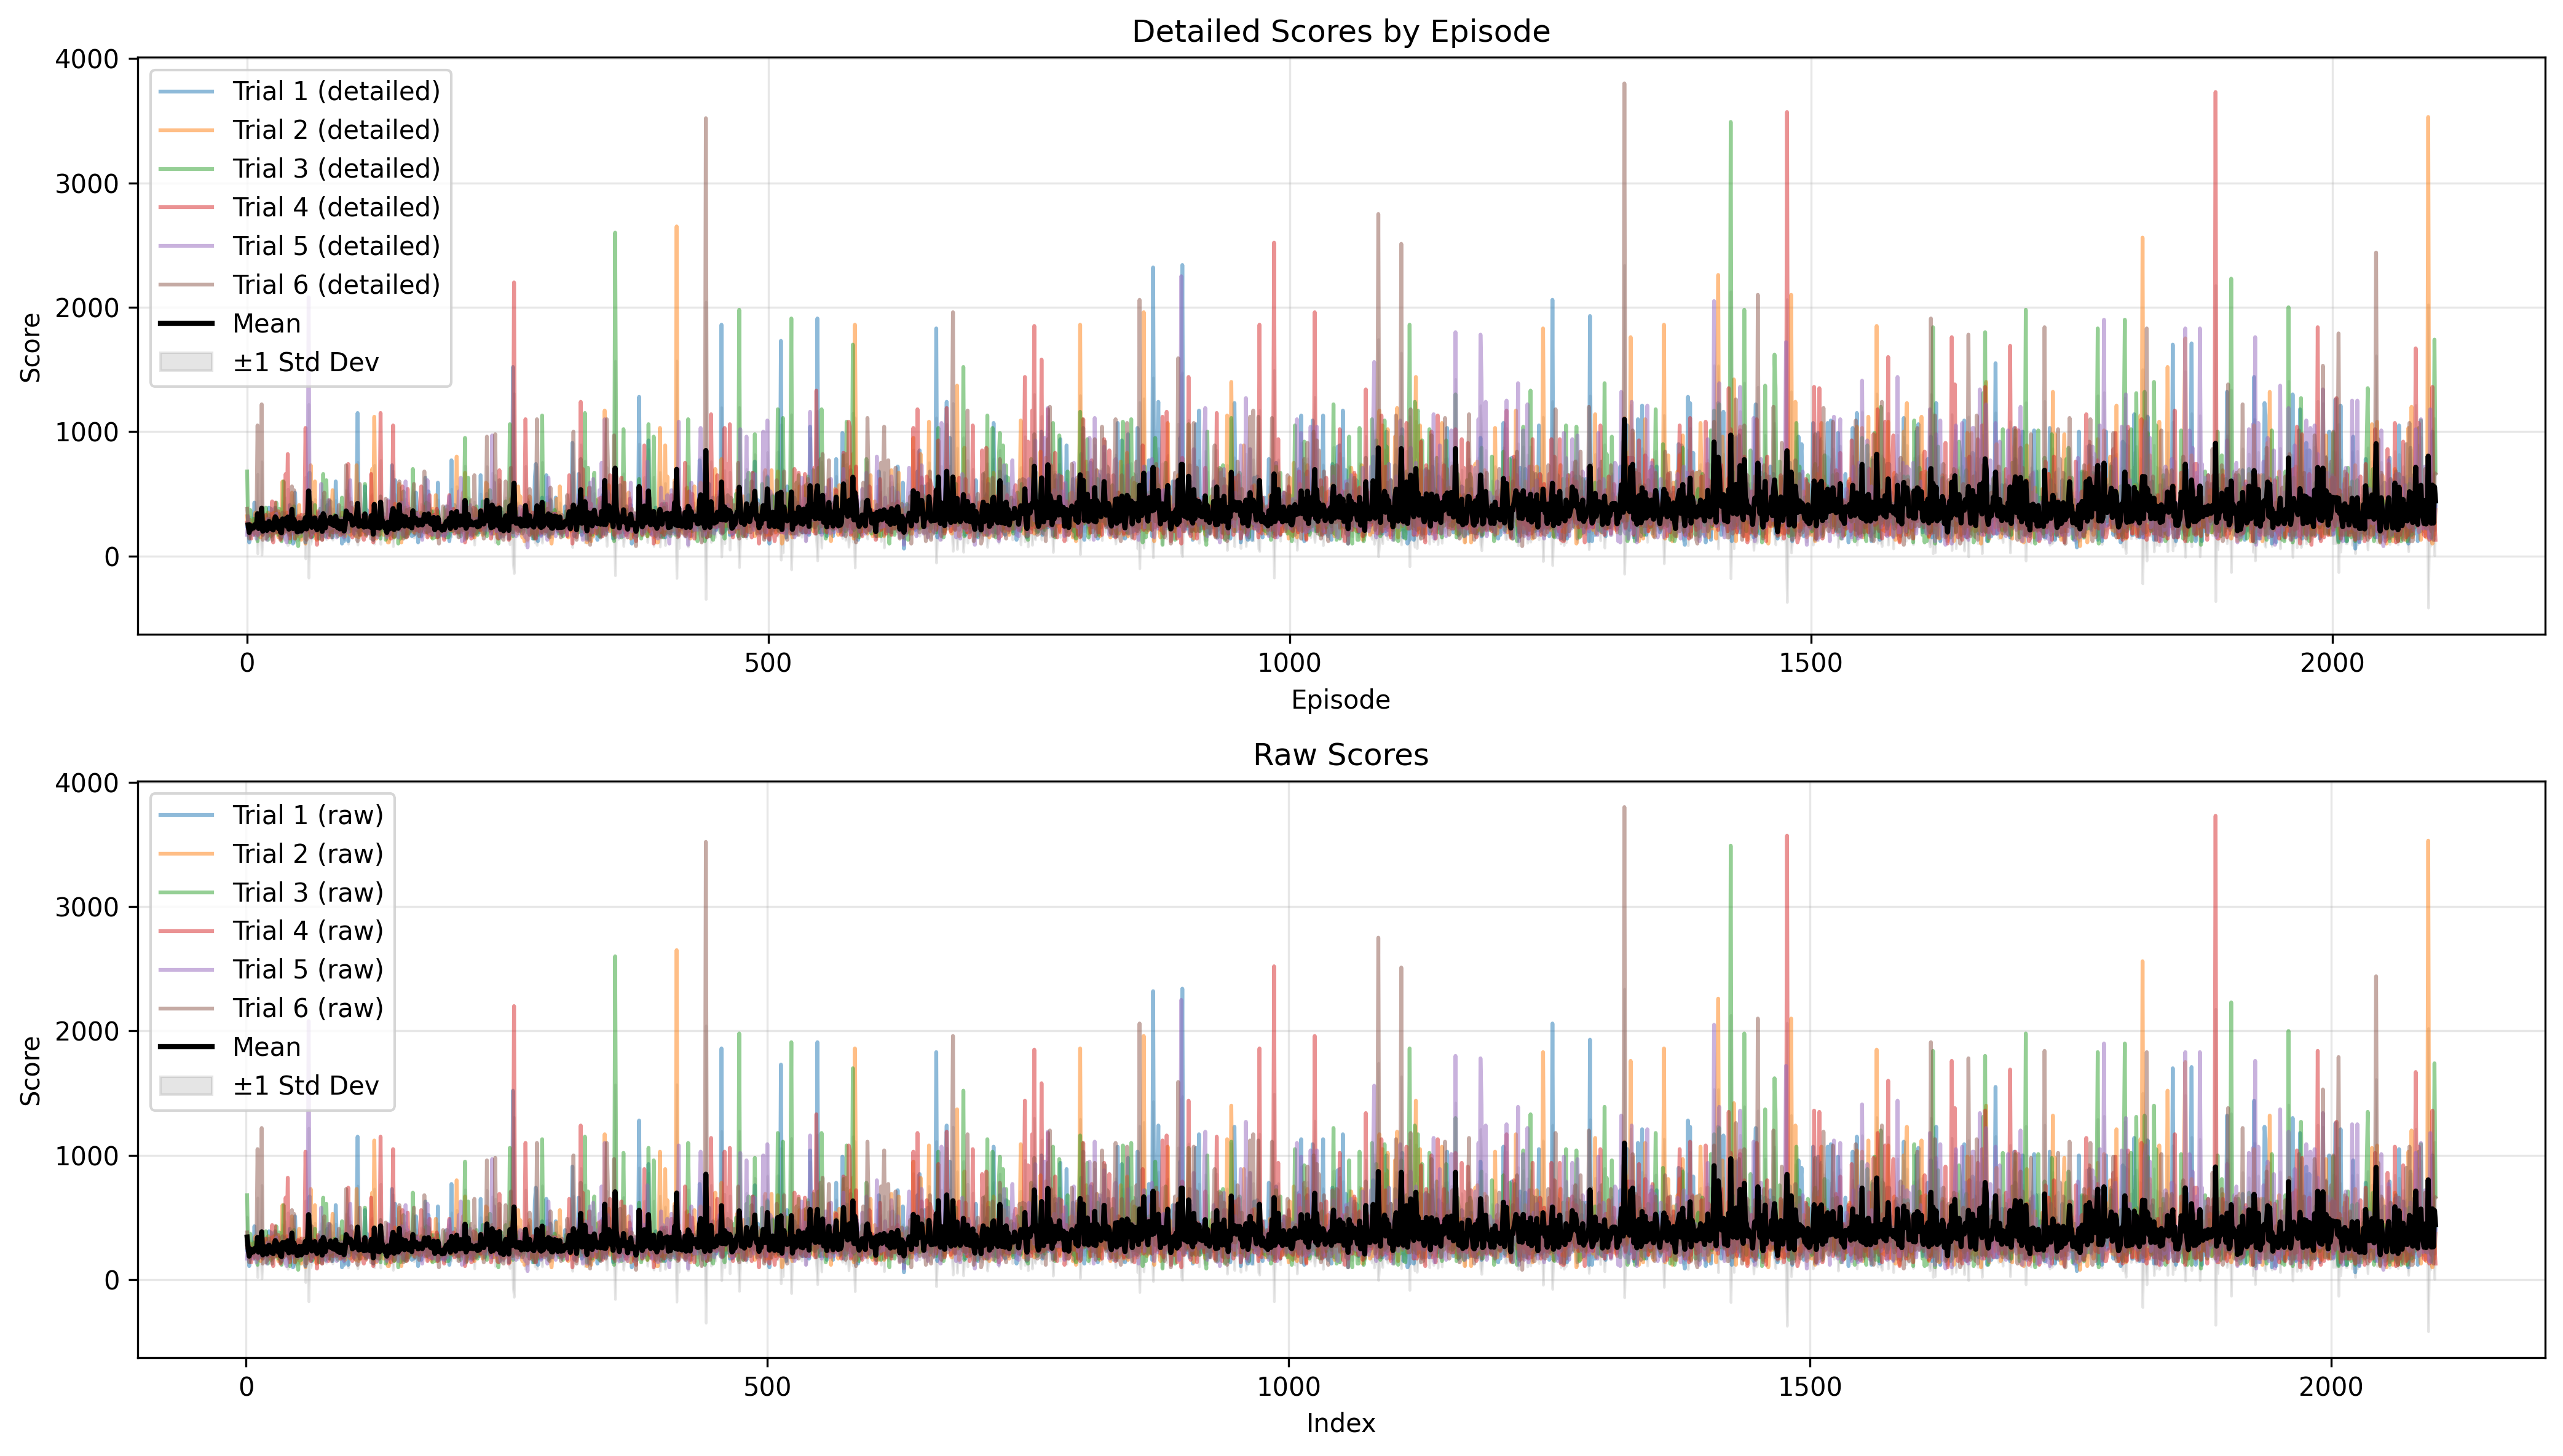
\includegraphics[width=0.8\textwidth]{../exp_1/images/score_analysis.png}
  \caption{Learning curve for Standard DQN (exp\_1). The plot shows the score progression over episodes, with multiple trials and the mean performance with standard deviation bands.}
  \label{fig:standard_dqn}
\end{figure}

\begin{figure}[h]
  \centering
  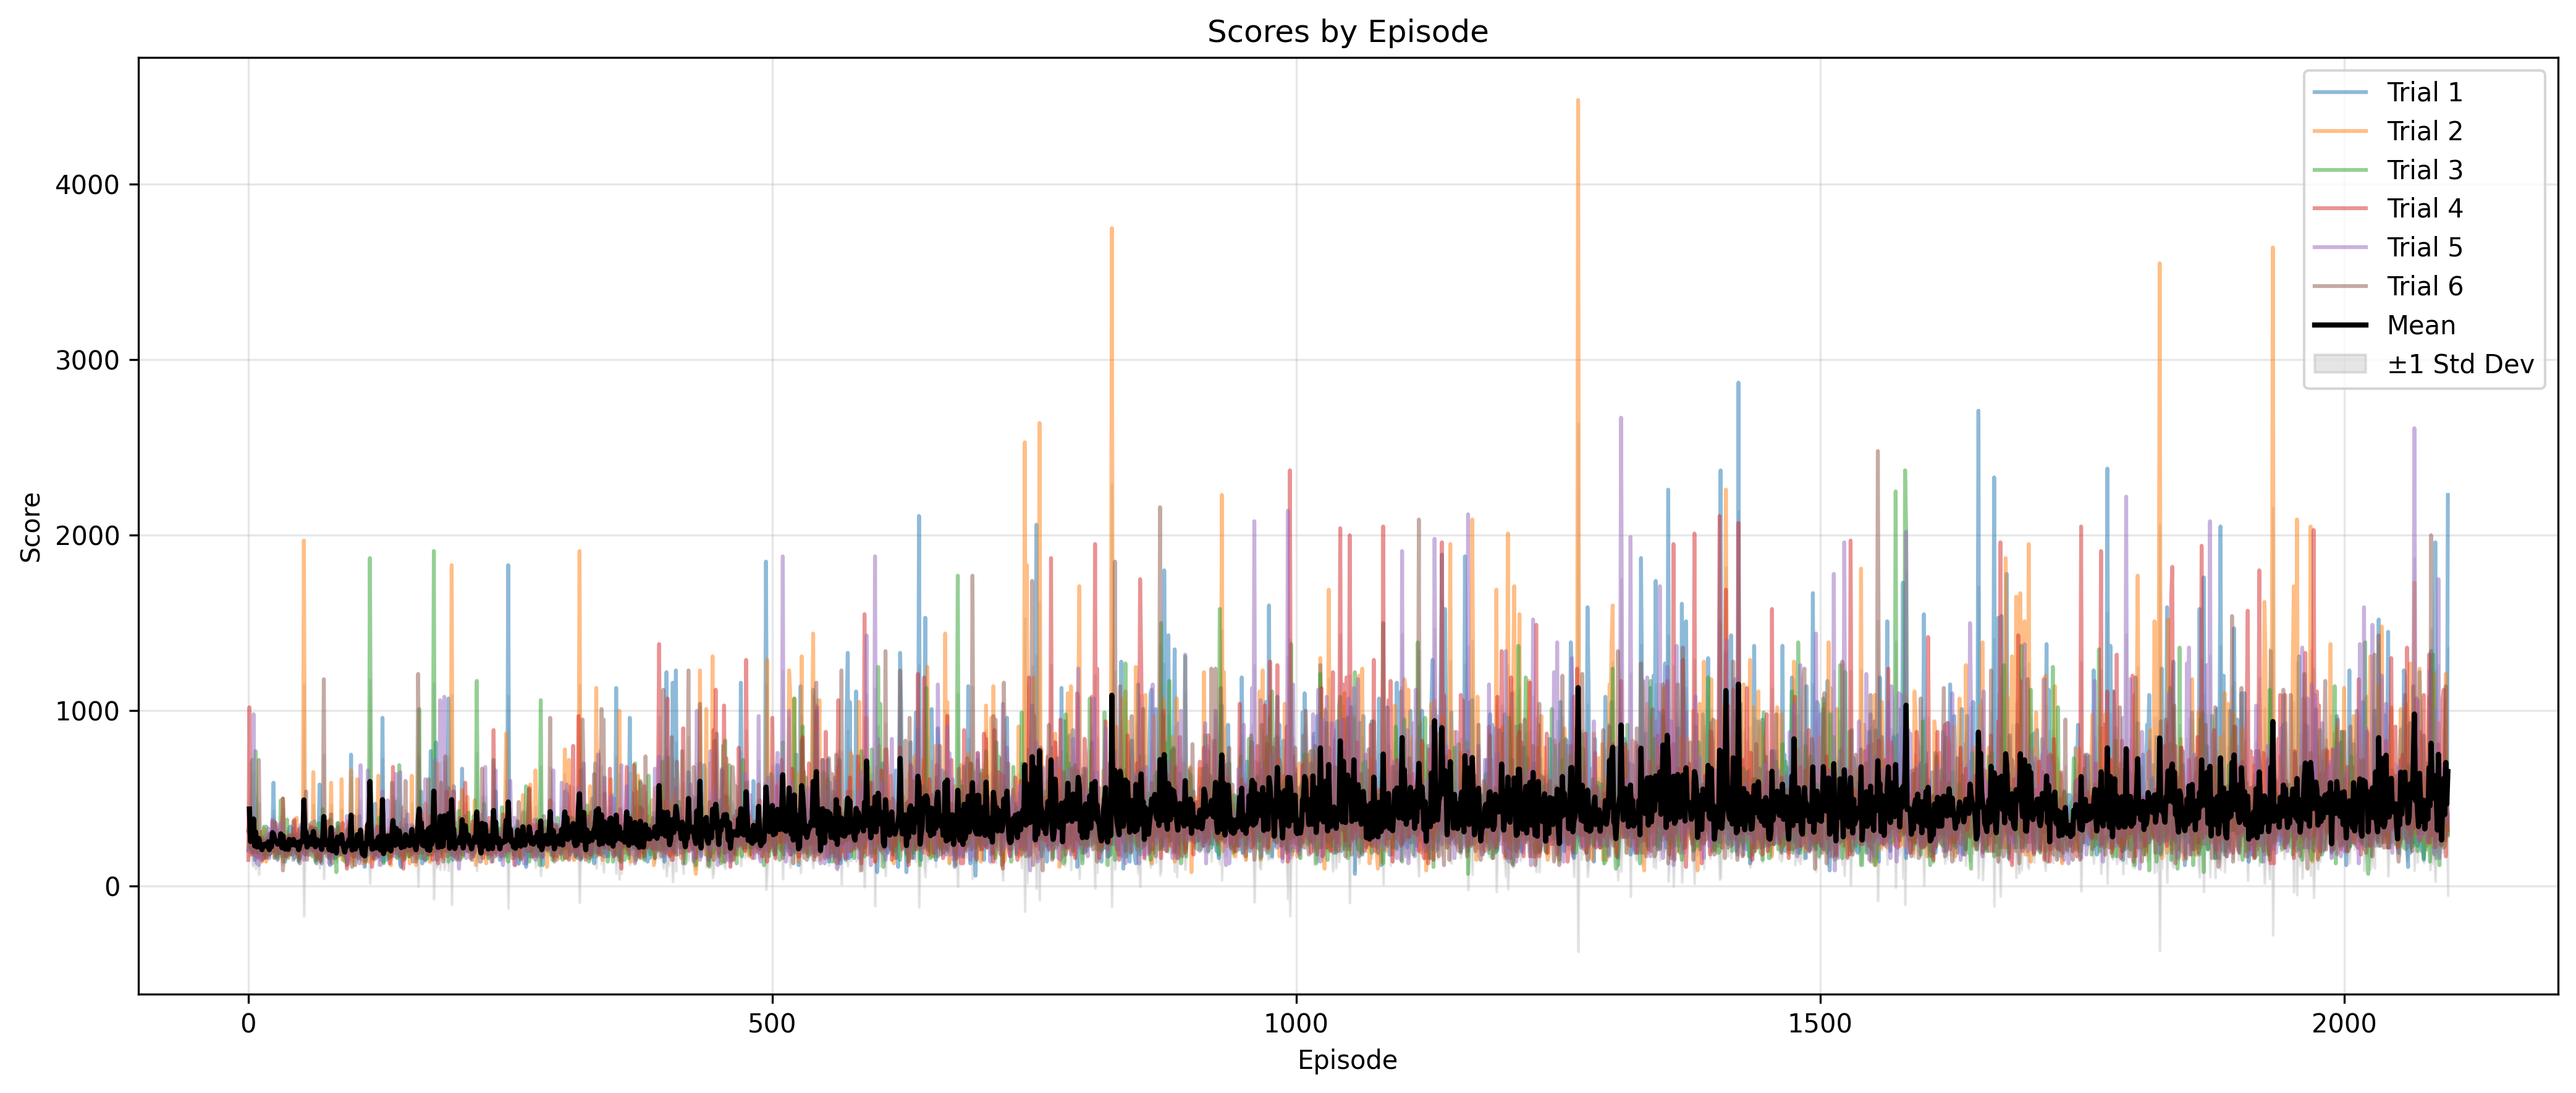
\includegraphics[width=0.8\textwidth]{../exp_2/images/score_analysis.png}
  \caption{Learning curve for Categorical Double DQN (exp\_2). The plot shows the score progression over episodes, with multiple trials and the mean performance with standard deviation bands.}
  \label{fig:cat_double_dqn}
\end{figure}

Our analysis revealed several key findings:

\begin{itemize}
  \item \textbf{Average Score}: The Categorical Double DQN achieved a higher average score (approximately 520 points) compared to the standard DQN (approximately 450 points), representing a 15.5\% improvement.

  \item \textbf{Maximum Score}: The improved model reached a maximum score of approximately 1,500 points, which is significantly higher than the standard DQN's maximum score of around 950 points.

  \item \textbf{Learning Stability}: The learning curve for the Categorical Double DQN shows more consistent improvement over time, with smaller fluctuations in performance compared to the standard DQN. This suggests that the distributional approach combined with double Q-learning provides more stable learning.

  \item \textbf{Learning Efficiency}: The improved model reached higher performance levels earlier in the training process, demonstrating better sample efficiency.
\end{itemize}

The standard deviation in scores was also lower for the Categorical Double DQN model, indicating more consistent performance across episodes. This suggests that the distributional approach helps the agent develop more robust policies that perform well across various game states.

\subsection{Ghost Behavior Adaptation}

To evaluate the adaptability of our models to different ghost behaviors, we tested both the standard DQN and the Categorical Double DQN on environments with modified ghost behavior patterns. We categorized the ghost behaviors into two types:

\begin{itemize}
  \item \textbf{Easy}: Ghosts with more predictable movement patterns and less aggressive pursuit strategies.
  \item \textbf{Hard}: Ghosts with more complex, aggressive behavior that actively target Pac-Man with better pathfinding algorithms.
\end{itemize}

Figure \ref{tab:ghost_adaptation} shows the performance of both models across the different ghost behavior settings.

\begin{table}[h]
  \centering
  \begin{tabular}{|l|c|c|c|c|}
    \hline
    \textbf{Model}         & \textbf{Environment} & \textbf{Avg. Score} & \textbf{Min Score} & \textbf{Max Score} \\
    \hline
    Standard DQN           & Easy                 & 519.25              & 120.0              & 2650.0             \\
    Standard DQN           & Hard                 & 122.33              & 60.0               & 1010.0             \\
    \hline
    Categorical Double DQN & Easy                 & 694.88              & 130.0              & 3750.0             \\
    Categorical Double DQN & Hard                 & 195.30              & 60.0               & 3210.0             \\
    \hline
  \end{tabular}
  \caption{Performance comparison of Standard DQN and Categorical Double DQN models across different ghost behavior patterns}
  \label{tab:ghost_adaptation}
\end{table}

Our analysis revealed several key observations regarding the models' adaptation capabilities:

\begin{itemize}
  \item \textbf{Performance Degradation}: Both models experienced significant performance drops when transitioning from easy to hard ghost behaviors. The standard DQN's average score decreased by 76.4\% (from 519.25 to 122.33), while the Categorical Double DQN's average score decreased by 71.9\% (from 694.88 to 195.30).

  \item \textbf{Relative Advantage}: The Categorical Double DQN maintained its performance advantage over the standard DQN across both environments. In the easy environment, it outperformed the standard DQN by 33.8\%, and in the hard environment, the advantage increased to 59.6\%.

  \item \textbf{Robustness}: The Categorical Double DQN showed greater robustness to environmental changes, as evidenced by both its higher average scores and its ability to achieve substantially higher maximum scores in both environments. Most notably, in the hard environment, the Categorical Double DQN reached a maximum score of 3210.0, which is more than three times the maximum score achieved by the standard DQN (1010.0).

  \item \textbf{Minimum Performance}: Both models had similar minimum scores across environments, suggesting that even advanced algorithms can struggle in particularly challenging game states.
\end{itemize}

These results suggest that the distributional approach combined with double Q-learning not only improves overall performance but also enhances the agent's ability to adapt to more challenging and unfamiliar ghost behaviors. The maintained performance advantage in harder environments indicates that the Categorical Double DQN develops more generalizable policies that can better handle variations in opponent behavior.


\section{Discussion}

Our experiments with standard DQN and Categorical Double DQN models in the Pac-Man environment provide key insights into reinforcement learning algorithms' capabilities when faced with changing environments.

The consistent performance advantage of the Categorical Double DQN (15.5\% improvement in average score and significantly higher maximum scores) aligns with previous findings on distributional approaches \cite{bellemare2017distributional}. This improvement likely stems from three key mechanisms: (1) enhanced risk-awareness through modeling outcome distributions rather than just expected values, (2) reduced overestimation bias via the Double DQN mechanism, and (3) improved state space exploration by capturing return uncertainty. The lower standard deviation in performance further indicates that distributional approaches produce more consistent and reliable policies.

Our ghost behavior adaptation experiments revealed that while both models experienced substantial performance drops when transitioning to harder environments (76.4\% decrease for standard DQN, 71.9\% for Categorical Double DQN), the Categorical Double DQN maintained and even increased its relative advantage (from 33.8\% in easy environments to 59.6\% in hard ones). Most notably, its maximum score in the hard environment (3210.0) was more than triple that of the standard DQN (1010.0), demonstrating superior capability to discover effective strategies in challenging scenarios.

From a cognitive perspective, our results parallel human learning patterns: initial steep improvement curves followed by gradual progress, difficulty transferring skills to more challenging environments, and performance variability across trials. The superior adaptability of the Categorical Double DQN resembles how humans with robust mental models better adapt to changing task parameters.

Our study has several limitations: the use of RAM-based representations rather than pixel inputs, limited environmental variations beyond ghost behaviors, finite training duration (2,100 episodes), and fixed hyper-parameters for each model.

Beyond Pac-Man, these findings have broader implications for reinforcement learning applications in dynamic environments, safety-critical systems requiring reliable behavior, and scenarios where sample efficiency is crucial. Our results support the hypothesis that advanced DQN variants develop more robust, adaptable policies—essential for artificial agents operating in unpredictable real-world environments.

\section{Next Steps}

Building upon the promising results of our current study, several directions for future research could further enhance our understanding of reinforcement learning in dynamic environments and improve the adaptability of agents in Pac-Man and similar domains:

\subsection{Algorithm Enhancements}

\begin{itemize}
  \item \textbf{Full Rainbow Implementation}: Integrate the remaining components of Rainbow DQN, including prioritized experience replay, multi-step learning, and noisy networks, to potentially achieve even better performance and adaptability.

  \item \textbf{Alternate Distributional Approaches}: Explore other distributional reinforcement learning methods such as Quantile Regression DQN (QR-DQN) or Implicit Quantile Networks (IQN), which might offer different advantages in capturing return distributions.

  \item \textbf{Meta-Learning}: Implement meta-learning approaches that explicitly optimize for fast adaptation to new environments, potentially enabling more rapid adjustment to changes in ghost behavior.
\end{itemize}

\subsection{Technical Improvements}

\begin{itemize}
  \item \textbf{Hyperparameter Optimization}: Conduct systematic hyperparameter tuning using Bayesian optimization or other advanced methods to find optimal settings for each algorithm.

  \item \textbf{Computational Efficiency}: Optimize implementation to reduce training time, enabling longer training periods and more comprehensive experiments across a wider range of conditions.

  \item \textbf{Transfer Learning}: Explore whether pre-training on standard ghost behaviors can accelerate adaptation to new ghost behaviors through fine-tuning approaches.
\end{itemize}

These future directions would extend our current findings and contribute to the broader goal of developing reinforcement learning agents that can robustly adapt to changing environments, a capability essential for real-world applications beyond game-playing domains.

\bibliography{iclr2021_conference}
\bibliographystyle{iclr2021_conference}

\end{document}
